Method Multiplication uses the technique of the decomposition of the API into multiple interface methods.
Decomposition could be done by responsibility, functionality, parameter types, or for example
nullability of some parameters.
The decomposition of the API into multiple interface methods is usually a trade-off between the usability and
the complexity of the API\@ - the functionality should not too fine-grained or vice-versa spanned over
multiple interface methods.

The Figure~\ref{fig:mult_decomposition_by_type} shows the decomposition of the API by the IGMPv2 types - the previous
version (Figure~\ref{fig:sing_write_max_response_time}) is split into 3 interface methods, one for each message type
\footnote{The next diagrams do not contain calculation of the checksum since it is not relevant for the demonstration
of API design and this process repeats in every version of example.}.
This allows us to remove the \textit{igmpType} parameter from the interface method and simplify checking of the input
parameters in the implementation logic.

\begin{figure}[!htb]
    \centering
    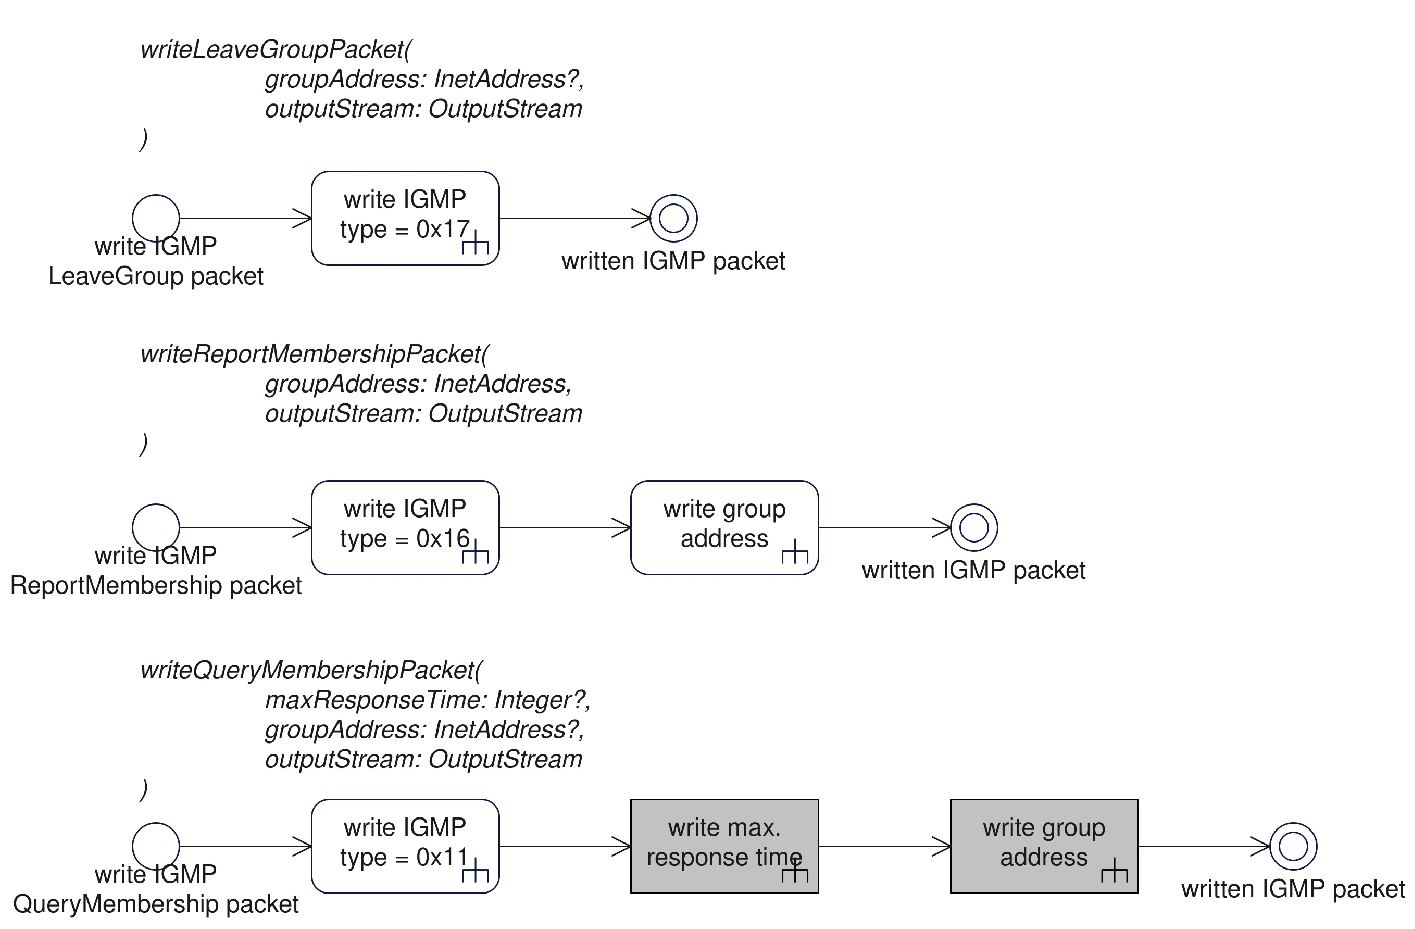
\includegraphics[width=1.0
    \textwidth]{mult_decomposition_by_type}
    \caption{Method Multiplication: Decomposition of API by type}
    \label{fig:mult_decomposition_by_type}
\end{figure}

In the previous Figure~\ref{fig:mult_decomposition_by_type} writing of the IGMP QueryMembership message is still
complex because there are 2 optional parameters \textit{maxResponseTime} and \textit{groupAddress}.
The group address is \textit{0.0.0.0} only in the case of the General Query message, otherwise, it is a mandatory
parameter - it makes sense to split the interface method into 2 interface methods - one for the General Query
message and another for the Group-Specific Query message.
This decomposition is shown in the Figure~\ref{fig:mult_decomposition_by_function}.

\begin{figure}[!htb]
    \centering
    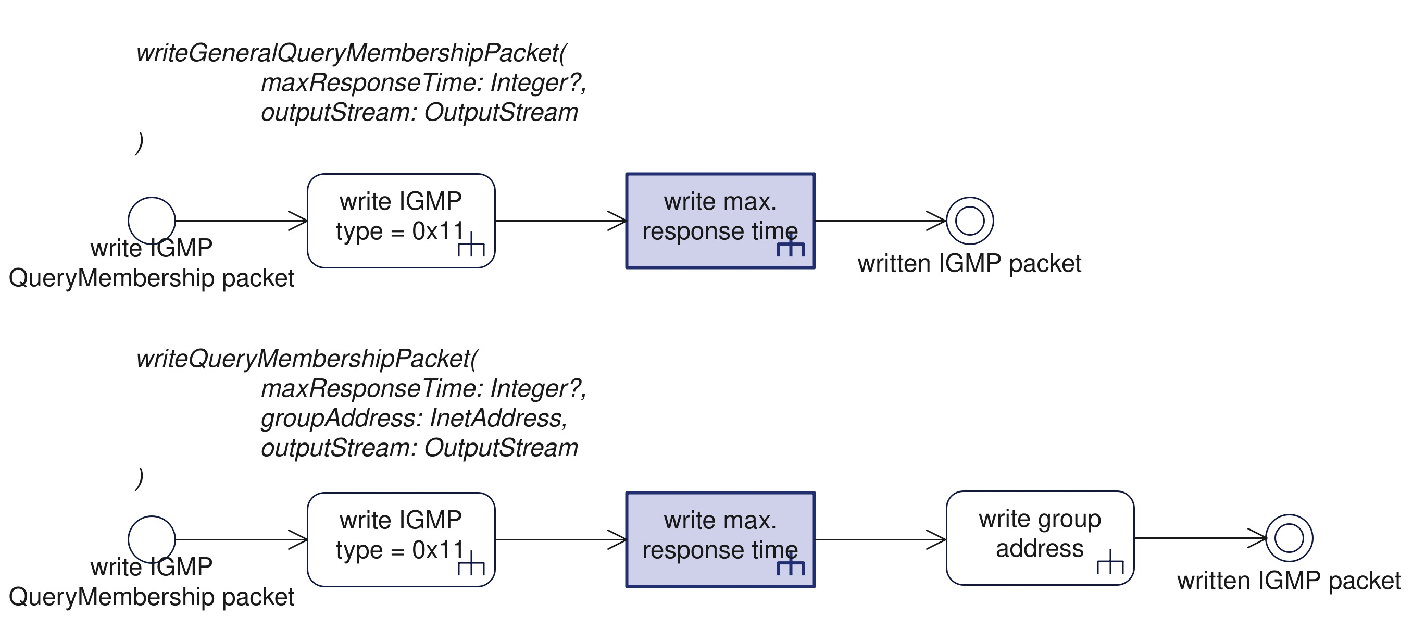
\includegraphics[width=1.0
    \textwidth]{mult_decomposition_by_function}
    \caption{Method Multiplication: Decomposition of API by functionality}
    \label{fig:mult_decomposition_by_function}
\end{figure}

Finally, the Figure~\ref{fig:mult_decomposition_by_default_values} shows splitting of the method for writing
QueryMembership message into 2 overloaded interface methods - one with the \textit{maxResponseTime} parameter and
another without it that internally sets some default value.
Note that method overloading is not possible in all programming languages, and it should not be used if methods
have the different functionality - in this case it is more readable to choose different identifiers for the methods.

\begin{figure}[!htb]
    \centering
    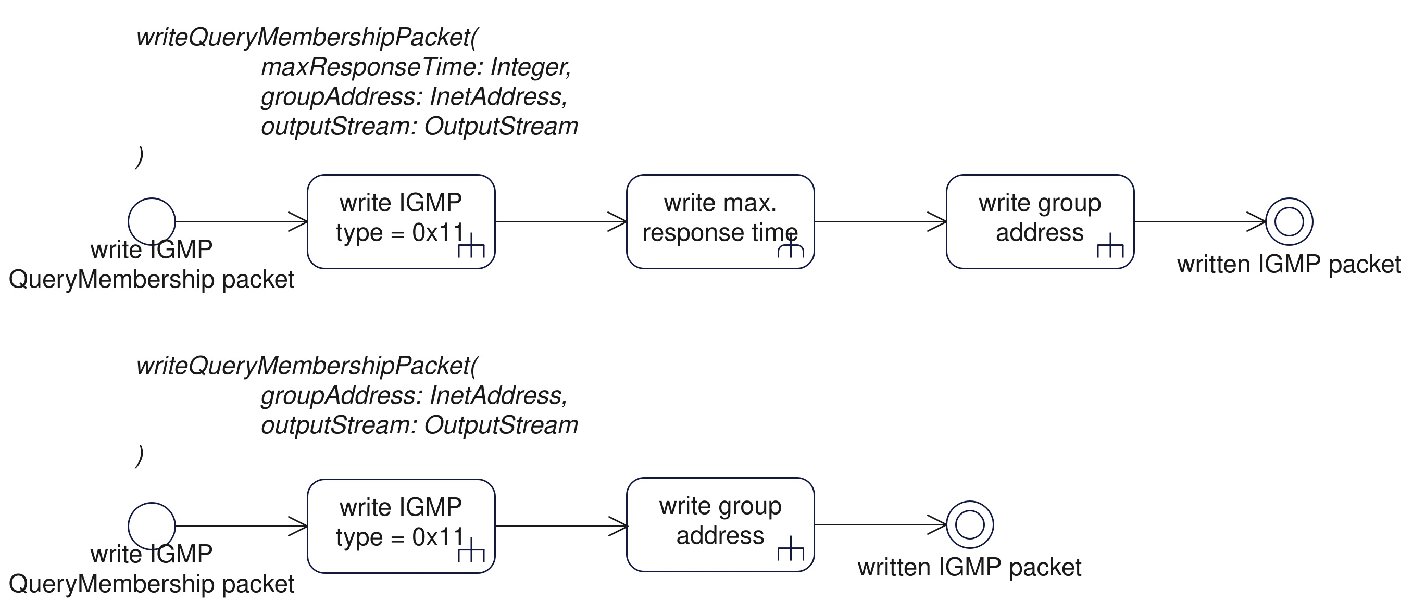
\includegraphics[width=1.0
    \textwidth]{mult_decomposition_by_default_values}
    \caption{Method Multiplication: Decomposition of API by default values}
    \label{fig:mult_decomposition_by_default_values}
\end{figure}

Benefits of the Method Multiplication:

\begin{itemize}
    \item The API is more readable and understandable than in case of Singleton Interface Method.
    If identifiers of interface methods are chosen correctly, it is easy to understand what is the purpose of the
    API method (code is often self-documented).
    \item Maintainability of the API is improved - It is easier to update or add new functionality to the API\@
    since changes are localized to the single interface method.
    \item API is more robust - It is not possible to call the method with invalid combination of the parameters.
    \item It is possible to get rid of God Methods - Implementation of the API is also split into multiple methods.
\end{itemize}

Drawbacks of the Method Multiplication:

\begin{itemize}
    \item Appearance of the God Classes - There is still a single service that is implemented by some class.
    Such implementation tends to grow over time and accumulate more and more functionality.
    In this case, further division of the service into multiple services may be beneficial, if it is possible
    to break service by functionality into smaller components (application of Vertical Slicing).
    \item Client must decide which method to call - In this case, there is usually another Facade layer on top
    of the API that hides the logic around calling of the correct interface method.
    This layer must be implemented and maintained.
    \item God Classes may host Spaghetti Code - It is characterized by a lack of structure or organization,
    often resulting from code that has been written in a hurry, without proper planning, or by a developer
    with a limited understanding of the software's structure.
    This can lead to a program with a complex and tangled control structure.
    Figure~\ref{fig:mult_spaghetti_code} shows an example of the Spaghetti Code in the early stage.
    There are multiple shared procedures that are called by API methods in a sequence with the unclear control flow.
    Internal functions tend to contain a lot of parameters that are passed between them.
    \item API Rooting - Implementations of the interface methods just call another common method that could be internal
    or even represented by another public interface method.
    That means that the API is decomposed but internal implementation stays to be implemented
    in Singleton Interface Method.
    Figure~\ref{fig:mult_api_rooting} shows an example of the API Rooting.
\end{itemize}

\begin{figure}[!htb]
    \centering
    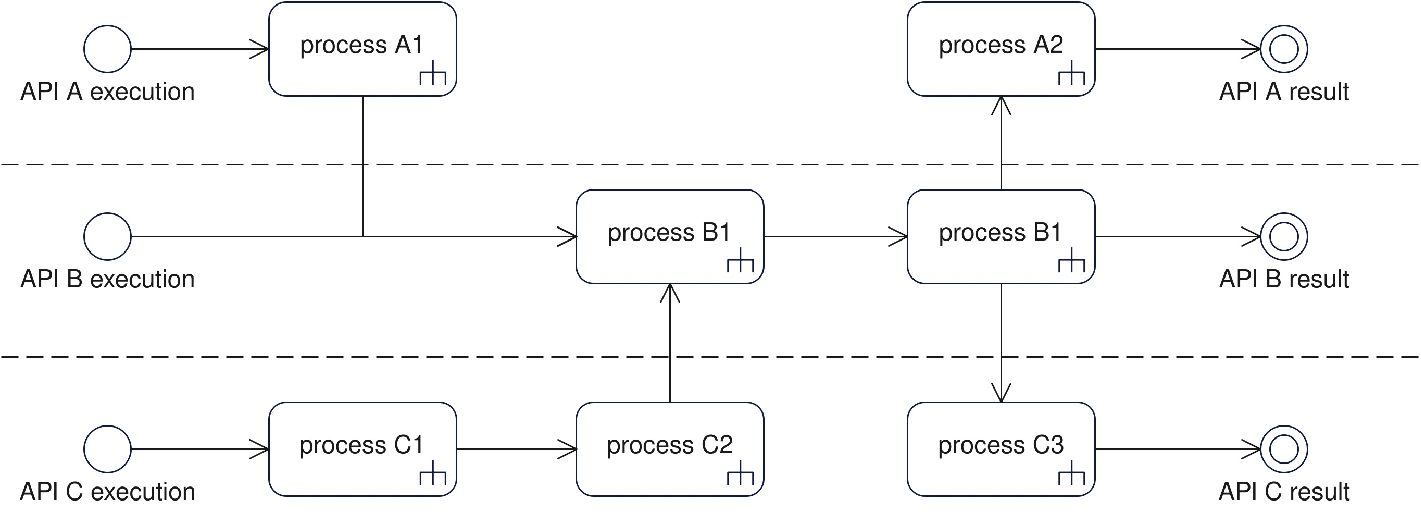
\includegraphics[width=1.0
    \textwidth]{mult_spaghetti_code}
    \caption{Method Multiplication: Germ of the Spaghetti Code}
    \label{fig:mult_spaghetti_code}
\end{figure}

\begin{figure}[!htb]
    \centering
    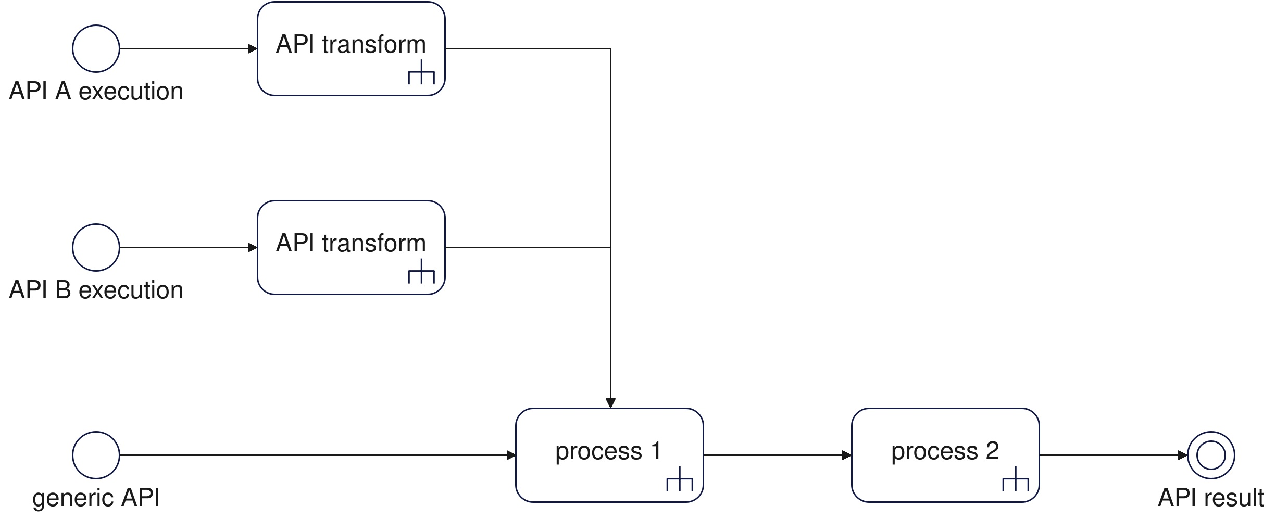
\includegraphics[width=1.0
    \textwidth]{mult_api_rooting}
    \caption{Method Multiplication: API Rooting}
    \label{fig:mult_api_rooting}
\end{figure}

Common use-cases of the Method Multiplication:

\begin{itemize}
    \item Decomposition of the API by the functionality into multiple interface methods.
    \item Overloading of the interface methods with the goal to support different types of the input parameters.
\end{itemize}
